

\newgeometry{top=1.5cm, bottom=1cm, left=1cm, right=1cm} 
\large

\begin{minipage}{.44\textwidth}
    \begin{center}
        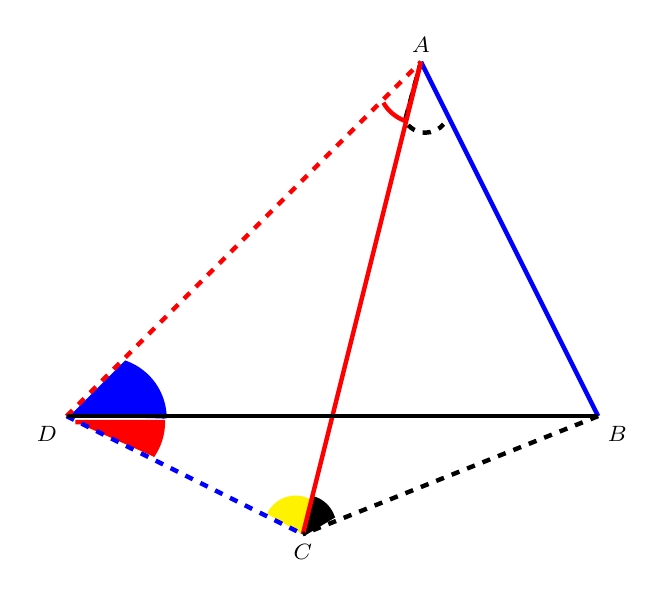
\begin{tikzpicture}[scale=0.75]
            \draw[red,ultra thick] (0,-2) -- (-0.27,-3) arc (70:30:-0.7);
            \draw[black,ultra thick, dashed] (0,-2) -- (-0.27,-3) arc (30:140:-0.4);
            \draw[fill=blue,ultra thick, blue] (-5.9,-8) -- (-5,-7.1) arc (70:0:1);
            \draw[fill=red,ultra thick, red] (-5.85,-8.1) -- (-4.37,-8.1) arc (360:325:1);
            \draw[fill=yellow,ultra thick, yellow] (-2, -10) -- (-1.8 , -9.5) arc (50:155:0.5);
            \draw[fill=black,ultra thick, black] (-2, -10) -- (-1.5 , -9.7) arc (20:75:0.5);
            \draw[dashed, ultra thick, red] (-6,-8) -- (0,-2);
            \draw[thick, ultra thick, blue] (0,-2) -- (3,-8);
            \draw[thick, ultra thick, red] (0,-2) -- (-2,-10);
            \draw[dashed, ultra thick, blue] (-6,-8) -- (-2,-10);
            \draw[dashed, ultra thick, black] (3, -8) -- (-2,-10);
            \draw[thick, ultra thick, black] (-6,-8) -- (3,-8);
            \node[above] at (0,-2) {\color{black}\footnotesize$A$};
            \node[below right] at (3,-8) {\color{black}\footnotesize$B$};
            \node[below] at (-2,-10) {\color{black}\footnotesize$C$};
            \node[below left] at (-6,-8) {\color{black}\footnotesize$D$};
        \end{tikzpicture}
    \end{center}
        \begin{center}
        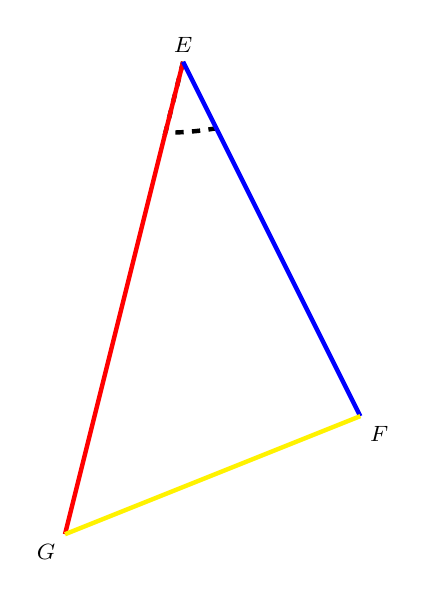
\begin{tikzpicture}[scale=0.75]
            \draw[dashed, ultra thick] (0,-2) -- (-0.3,-3.2) arc (90:100:-5);
            \draw[ultra thick, -, red] (-2,-10) -- (0,-2);
            \draw[ultra thick, -, blue] (0,-2) -- (3,-8);
            \draw[ultra thick, -, yellow] (-2,-10) -- (3,-8);
            \node[below left] at (-2,-10) {\color{black}\footnotesize$G$};
            \node[above] at (0,-2) {\color{black}\footnotesize$E$};
            \node[below right] at (3,-8) {\color{black}\footnotesize$F$};
        \end{tikzpicture}
    \end{center}
\end{minipage}
\hfill
\begin{minipage}{.55\textwidth}
    \begin{flushright}
       \ \ \textit{48} \ \ \ \ \ \Large{КНИГА I ПРЕДЛ.XXIV.ТЕОРЕМА} \
    \end{flushright}\\

    \begin{minipage}{.2\textwidth}
        
\includegraphics[width=1\textwidth]{images/E.png}
    \end{minipage}
    \hfill
    \begin{minipage}{.79\textwidth}
        \textit{сли у двух треугольников по две стороны со\-ответственно равны друг другу(}
        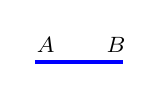
\begin{tikzpicture}[scale=0.75]
            \draw[ultra thick, -, blue] (0,0) -- (1.5,0);
            \node[above left] at (0.5,0) {\color{black}\footnotesize$A$};
            \node[above left] at (1.7,0) {\color{black}\footnotesize$B$};
        \end{tikzpicture}
        \textit{=}
        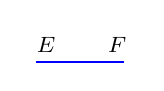
\begin{tikzpicture}[scale=0.75]
            \draw[thick, -, blue] (0,0) -- (1.5,0);
            \node[above left] at (0.5,0) {\color{black}\footnotesize$E$};
            \node[above left] at (1.7,0) {\color{black}\footnotesize$F$};
        \end{tikzpicture}
        \textit{и}
        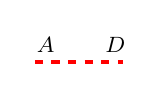
\begin{tikzpicture}[scale=0.75]
            \draw[ultra thick, dashed, red] (0,0) -- (1.5,0);
            \node[above left] at (0.5,0) {\color{black}\footnotesize$A$};
            \node[above left] at (1.7,0) {\color{black}\footnotesize$D$};
        \end{tikzpicture}
        \textit{=}
        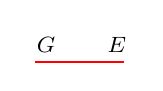
\begin{tikzpicture}[scale=0.75]
            \draw[thick, -, red] (0,0) -- (1.5,0);
            \node[above left] at (0.5,0) {\color{black}\footnotesize$G$};
            \node[above left] at (1.7,0) {\color{black}\footnotesize$E$};
        \end{tikzpicture}
        \textit{), и угол за-}
    \end{minipage}
    \vspace{1pt}
    \begin{minipage}{.45\textwidth}
        \textit{ключенный ними в одном}
    \end{minipage}
    \begin{minipage}{.1\textwidth}
        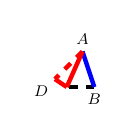
\begin{tikzpicture}[scale=0.5]
            \draw[ultra thick, dashed, black] (0.7,-0.5) -- (0,-0.5);
            \draw[ultra thick, -, blue] (0.4,0.4) -- (0.7,-0.5);
            \draw[ultra thick, -, red] (0.4,0.4) -- (0,-0.5);
            \draw[ultra thick, dashed, red] (0.4,0.4) -- (-0.3,-0.3);
            \draw[ultra thick, -, red] (0,-0.5) -- (-0.3,-0.3);
            \node[above, scale=0.7 ] at (0.4,0.4) {\color{black}\footnotesize$A$};
            \node[below, scale=0.7] at (0.7,-0.5) {\color{black}\footnotesize$B$};
            \node[below left, scale=0.7] at (-0.3,-0.3) {\color{black}\footnotesize$D$};
        \end{tikzpicture}
    \end{minipage}
    \begin{minipage}{.43\textwidth}
       \textit{больше, чем в другом}
    \end{minipage}


    
    \begin{minipage}{.1\textwidth}
        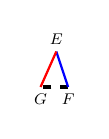
\begin{tikzpicture}[scale=0.5]
            \draw[ultra thick, dashed, black] (0.7,-0.5) -- (0,-0.5);
            \draw[thick, -, blue] (0.4,0.4) -- (0.7,-0.5);
            \draw[thick, -, red] (0.4,0.4) -- (0,-0.5);
            \node[above, scale=0.7 ] at (0.4,0.4) {\color{black}\footnotesize$E$};
            \node[below, scale=0.7] at (0.7,-0.5) {\color{black}\footnotesize$F$};
            \node[below, scale=0.7] at (0,-0.5) {\color{black}\footnotesize$G$};
        \end{tikzpicture}
    \end{minipage}
    \begin{minipage}{.9\textwidth}
       \textit{, то сторона}
        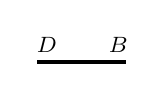
\begin{tikzpicture}[scale=0.75]
            \draw[ultra thick, -] (0,0) -- (1.5,0);
            \node[above left] at (0.5,0) {\color{black}\footnotesize$D$};
            \node[above left] at (1.7,0) {\color{black}\footnotesize$B$};
        \end{tikzpicture}
        \textit{противолежащая больше-}
    \end{minipage}
    \textit{му углу больше стороны, противолежащей меньшему}
    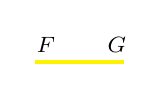
\begin{tikzpicture}[scale=0.75]
        \draw[ultra thick, -, yellow] (0,0) -- (1.5,0);
        \node[above left] at (0.5,0) {\color{black}\footnotesize$F$};
        \node[above left] at (1.7,0) {\color{black}\footnotesize$G$};
    \end{tikzpicture}
    .
    \begin{center}
       \ \ \ \ \ \ \
        \begin{center}
           Сделаем 
            \begin{minipage}{.1\textwidth}
                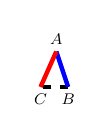
\begin{tikzpicture}[scale=0.5]
                    \draw[ultra thick, dashed, black] (0.7,-0.5) -- (0,-0.5);
                    \draw[ultra thick, -, blue] (0.4,0.4) -- (0.7,-0.5);
                    \draw[ultra thick, -, red] (0.4,0.4) -- (0,-0.5);
                    \node[above, scale=0.7 ] at (0.4,0.4) {\color{black}\footnotesize$A$};
                    \node[below, scale=0.7] at (0.7,-0.5) {\color{black}\footnotesize$B$};
                    \node[below, scale=0.7] at (0,-0.5) {\color{black}\footnotesize$C$};
                \end{tikzpicture}
            \end{minipage}
            =
            \begin{minipage}{.1\textwidth}
                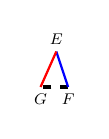
\begin{tikzpicture}[scale=0.5]
                    \draw[ultra thick, dashed, black] (0.7,-0.5) -- (0,-0.5);
                    \draw[thick, -, blue] (0.4,0.4) -- (0.7,-0.5);
                    \draw[thick, -, red] (0.4,0.4) -- (0,-0.5);
                    \node[above, scale=0.7 ] at (0.4,0.4) {\color{black}\footnotesize$E$};
                    \node[below, scale=0.7] at (0.7,-0.5) {\color{black}\footnotesize$F$};
                    \node[below, scale=0.7] at (0,-0.5) {\color{black}\footnotesize$G$};
                \end{tikzpicture}
            \end{minipage}
            (пр. I$._23$), \\
        \end{center}
        \begin{center}
            и
            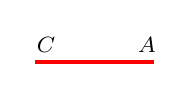
\begin{tikzpicture}[scale=0.75]
                \draw[ultra thick, -, red] (0,0) -- (2,0);
                \node[above left] at (0.5,0) {\color{black}\footnotesize$C$};
                \node[above left] at (2.2,0) {\color{black}\footnotesize$A$};
            \end{tikzpicture}
            =
            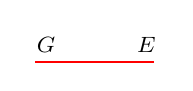
\begin{tikzpicture}[scale=0.75]
                \draw[thick, -, red] (0,0) -- (2,0);
                \node[above left] at (0.5,0) {\color{black}\footnotesize$G$};
                \node[above left] at (2.2,0) {\color{black}\footnotesize$E$};
            \end{tikzpicture}
            (пр. I$._3$), \\
        \end{center}
        \begin{center}
            проведём
            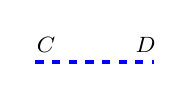
\begin{tikzpicture}[scale=0.75]
                \draw[ultra thick, dashed, blue] (0,0) -- (2,0);
                \node[above left] at (0.5,0) {\color{black}\footnotesize$C$};
                \node[above left] at (2.2,0) {\color{black}\footnotesize$D$};
            \end{tikzpicture}
            и
            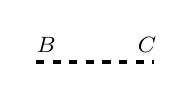
\begin{tikzpicture}[scale=0.75]
                \draw[ultra thick, dashed] (0,0) -- (2,0);
                \node[above left] at (0.5,0) {\color{black}\footnotesize$B$};
                \node[above left] at (2.2,0) {\color{black}\footnotesize$C$};
            \end{tikzpicture}
            . \\
        \end{center}
        \begin{center}
            Поскольку
            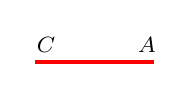
\begin{tikzpicture}[scale=0.75]
                \draw[ultra thick, -, red] (0,0) -- (2,0);
                \node[above left] at (0.5,0) {\color{black}\footnotesize$C$};
                \node[above left] at (2.2,0) {\color{black}\footnotesize$A$};
            \end{tikzpicture}
            =
            \begin{tikzpicture}[scale=0.75]
                \draw[thick, dashed, red] (0,0) -- (2,0);
                \node[above left] at (0.5,0) {\color{black}\footnotesize$A$};
                \node[above left] at (2.2,0) {\color{black}\footnotesize$D$};
            \end{tikzpicture}
            (акс. I, гип., постр.)\\
        \end{center}
        \begin{center}
            \begin{tikzpicture}
                \fill [black] (0, 0) circle (1pt);
                \fill [black] (0.1, -0.15) circle (1pt);
                \fill [black] (-0.1, -0.15) circle (1pt);
            \end{tikzpicture}
            \begin{minipage}{.1\textwidth}
                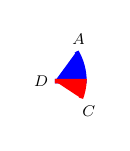
\begin{tikzpicture}[scale=0.75]
                    \draw[ultra thick, blue, fill=blue] (0,0) -- (0.5,0) arc (0:30:1);
                    \draw[ultra thick, red, fill=red] (0,0) -- (0.5,0) arc (-3:-20:1);
                    \node[above, scale=0.7] at (0.4,0.5) {\color{black}\footnotesize$A$};
                    \node[left, scale=0.7] at (0,0) {\color{black}\footnotesize$D$};
                    \node[below right, scale=0.7] at (0.35,-0.3) {\color{black}\footnotesize$C$};
                \end{tikzpicture}
            \end{minipage}
            =
            \begin{minipage}{.1\textwidth}
                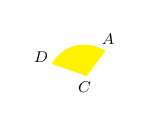
\begin{tikzpicture}[scale=0.75]
                    \draw[ultra thick, yellow, fill=yellow] (0,0) -- (0.3,0.4) arc (60:150:0.6);
                    \node[above, scale=0.7] at (0.4,0.4) {\color{black}\footnotesize$A$};
                    \node[left, scale=0.7] at (-0.5,0.3) {\color{black}\footnotesize$D$};
                    \node[below, scale=0.7] at (0,0) {\color{black}\footnotesize$C$};
                \end{tikzpicture}
            \end{minipage}
            (пр. I$._5$), но
            \begin{minipage}{.1\textwidth}
                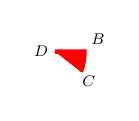
\begin{tikzpicture}[scale=0.75]
                    \draw[ultra thick, red, fill=red] (0,0) -- (0.5,0) arc (0:-20:1);
                    \node[above right, scale=0.7] at (0.5,0) {\color{black}\footnotesize$B$};
                    \node[left, scale=0.7] at (0,0) {\color{black}\footnotesize$D$};
                    \node[below right, scale=0.7] at (0.35,-0.3) {\color{black}\footnotesize$C$};
                \end{tikzpicture}
            \end{minipage}
            <
            \begin{minipage}{.1\textwidth}
                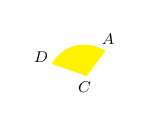
\begin{tikzpicture}[scale=0.75]
                    \draw[ultra thick, yellow, fill=yellow] (0,0) -- (0.3,0.4) arc (60:150:0.6);
                    \node[above, scale=0.7] at (0.4,0.4) {\color{black}\footnotesize$A$};
                    \node[left, scale=0.7] at (-0.5,0.3) {\color{black}\footnotesize$D$};
                    \node[below, scale=0.7] at (0,0) {\color{black}\footnotesize$C$};
                \end{tikzpicture}
            \end{minipage}
            ,\\
        \end{center}  
        \begin{center}
            и
            \begin{tikzpicture}
                \fill [black] (0, 0) circle (1pt);
                \fill [black] (0.1, -0.15) circle (1pt);
                \fill [black] (-0.1, -0.15) circle (1pt);
            \end{tikzpicture}
            \begin{minipage}{.1\textwidth}
                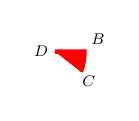
\begin{tikzpicture}[scale=0.75]
                    \draw[ultra thick, red, fill=red] (0,0) -- (0.5,0) arc (0:-20:1);
                    \node[above right, scale=0.7] at (0.5,0) {\color{black}\footnotesize$B$};
                    \node[left, scale=0.7] at (0,0) {\color{black}\footnotesize$D$};
                    \node[below right, scale=0.7] at (0.35,-0.3) {\color{black}\footnotesize$C$};
                \end{tikzpicture}
            \end{minipage}
            <
            \begin{minipage}{.1\textwidth}
                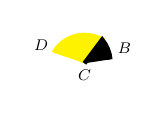
\begin{tikzpicture}[scale=0.75]
                    \draw[ultra thick, yellow, fill=yellow] (0,0) -- (0.3,0.4) arc (60:150:0.6);
                    \draw[ultra thick, black, fill=black] (0,0) -- (0.3,0.4) arc (-140:-175:-0.6);
                    \node[right, scale=0.7] at (0.45,0.25) {\color{black}\footnotesize$B$};
                    \node[left, scale=0.7] at (-0.5,0.3) {\color{black}\footnotesize$D$};
                    \node[below, scale=0.7] at (0,0) {\color{black}\footnotesize$C$};
                \end{tikzpicture}
            \end{minipage}
            \ \ 
            ,\\
        \end{center}
        \begin{center}
            \begin{tikzpicture}
                \fill [black] (0, 0) circle (1pt);
                \fill [black] (0.1, -0.15) circle (1pt);
                \fill [black] (-0.1, -0.15) circle (1pt);
            \end{tikzpicture}  
            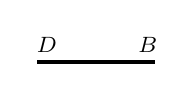
\begin{tikzpicture}[scale=0.75]
                \draw[ultra thick, -] (0,0) -- (2,0);
                \node[above left] at (0.5,0) {\color{black}\footnotesize$D$};
                \node[above left] at (2.2,0) {\color{black}\footnotesize$B$};
            \end{tikzpicture}
            >
            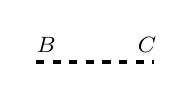
\begin{tikzpicture}[scale=0.75]
                \draw[ultra thick, dashed] (0,0) -- (2,0);
                \node[above left] at (0.5,0) {\color{black}\footnotesize$B$};
                \node[above left] at (2.2,0) {\color{black}\footnotesize$C$};
            \end{tikzpicture}    
            (пр. I$._19$)
        \end{center}
        \begin{center}
            но
            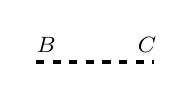
\begin{tikzpicture}[scale=0.75]
                \draw[ultra thick, dashed] (0,0) -- (2,0);
                \node[above left] at (0.5,0) {\color{black}\footnotesize$B$};
                \node[above left] at (2.2,0) {\color{black}\footnotesize$C$};
            \end{tikzpicture}   
            =
            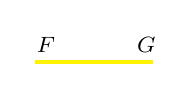
\begin{tikzpicture}[scale=0.75]
                \draw[ultra thick, -, yellow] (0,0) -- (2,0);
                \node[above left] at (0.5,0) {\color{black}\footnotesize$F$};
                \node[above left] at (2.2,0) {\color{black}\footnotesize$G$};
            \end{tikzpicture}  
            (пр. I$._4$)\\
        \end{center}
        \begin{center}
            \begin{tikzpicture}
                \fill [black] (0, 0) circle (1pt);
                \fill [black] (0.1, -0.15) circle (1pt);
                \fill [black] (-0.1, -0.15) circle (1pt);
            \end{tikzpicture} 
            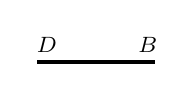
\begin{tikzpicture}[scale=0.75]
                \draw[ultra thick, -] (0,0) -- (2,0);
                \node[above left] at (0.5,0) {\color{black}\footnotesize$D$};
                \node[above left] at (2.2,0) {\color{black}\footnotesize$B$};
            \end{tikzpicture}     
            >
            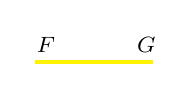
\begin{tikzpicture}[scale=0.75]
                \draw[ultra thick, -, yellow] (0,0) -- (2,0);
                \node[above left] at (0.5,0) {\color{black}\footnotesize$F$};
                \node[above left] at (2.2,0) {\color{black}\footnotesize$G$};
            \end{tikzpicture} 
            .
        \end{center}
    \end{center}
    \begin{flushright}
        ч.т.д.
    \end{flushright}
\end{minipage}
